\documentclass[11pt, reqno]{amsart}

\input{~/latex-common/macros.tex}
\usepackage[backend=bibtex,style=science]{biblatex}
% \bibliography{main.bib}
\pgfplotsset{compat=1.18}

\pagestyle{fancy}                         % fancy (allow headers, footers)
\fancyhf{}                                % clear all header/footer settings.
\cfoot{\thepage}                          % set page-numbers in footer.
% \lhead{\textit{\textbf{ Amittai, S}}}   % set name in header, left.
% \rhead{\textsc{Math 71: Algebra}}       % set class name in header, right.
\renewcommand{\headrulewidth}{0pt}
\renewcommand{\footrulewidth}{0pt}


\renewcommand{\theenumi}{\alph{enumi}}

\begin{document}

\newdate{due-date}{23}{05}{2023}

\title{CS-89.31: Deep Learning Generalization and Robustness\\ Amittai Siavava \\ \displaydate{due-date}}
\author{Amittai Siavava}
% \date{\today}


\setlength{\headheight}{13.0pt}
\setlength{\footskip}{15.0pt}

\maketitle

\bigskip

\def \cram { \textsc{cram} }
\def \dom { \textsc{domineering} }
\def \sub { \textsc{subtraction} }
\def \weighted { \textsc{weighted odds and evens}}
\def \nim { \textsc{nim} }
\def \P { \mathbf{P}}
\def \N { \mathbf{N}}

\section{Adversarial Training}

The adversarial training part was quite interesting.
I initially tried training on a MacBook Pro but it was taking too long (around $5$ minutes per epoch).
I then shifted to my Windows laptop which has a discrete graphics card, and the training time went
down to less than half a minute per epoch. The entire training still took around $90$ minutes,
but it was really interesting to see the model predictions improve.


\begin{figure}[h]
  \centering
  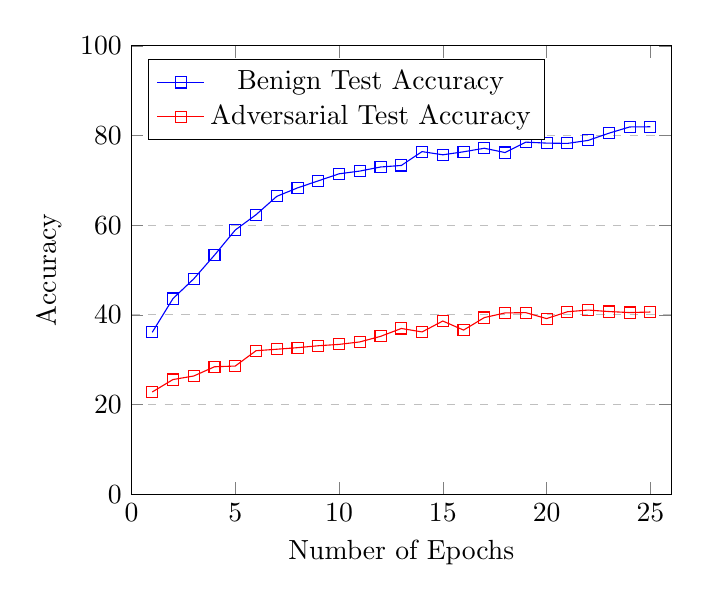
\begin{tikzpicture}
    \begin{axis}[
      xlabel={Number of Epochs},
      ylabel={Accuracy},
      xmin=0, xmax=26,
      ymin=0, ymax=100,
      xtick={0,5,10,15,20,25},
      ytick={0,20,40,60,80,100},
      legend pos=north west,
      ymajorgrids=true,
      grid style=dashed,
      ]
      \addplot[
      color=blue,
      mark=square,
      ]
      coordinates {
        (1,36.10)(2,43.62)(3,48.02)(4,53.31)(5,58.91)(6,62.32)(7,66.42)(8,68.31)(9,69.88)(10,71.45)(11,72.06)(12,72.97)(13,73.31)(14,76.40)(15,75.69)(16,76.36)(17,77.15)(18,76.19)(19,78.51)(20,78.30)(21,78.23)(22,78.90)(23,80.50)(24,81.90)(25,81.94)
      };
      \addlegendentry{Benign Test Accuracy}
      \addplot[
      color=red,
      mark=square,
      ]
      coordinates {
        (1,22.78)(2,25.56)(3,26.35)(4,28.41)(5,28.57)(6,31.99)(7,32.32)(8,32.67)(9,33.10)(10,33.40)(11,33.95)(12,35.19)(13,36.95)(14,36.18)(15,38.61)(16,36.59)(17,39.38)(18,40.42)(19,40.48)(20,39.15)(21,40.68)(22,41.06)(23,40.73)(24,40.50)(25,40.62)
      };
      \addlegendentry{Adversarial Test Accuracy}
    \end{axis}
  \end{tikzpicture}
  \caption{Adversarial Training Results (Graph).}~\label{fig:results}
\end{figure}

\newpage


\begin{table}[h]
    \centering
    \begin{tabular}{| r | r | r |}
      \bottomrule
      \textbf{Number of Epochs}   & \textbf{Benign Test Accuracy}  & \textbf{Adversarial Test Accuracy} \\   
      \midrule
      $1$                         & $36.10$                 & $22.78$ \\
      $2$                         & $43.62$                 & $25.56$ \\
      $3$                         & $48.02$                 & $26.35$ \\
      $4$                         & $53.31$                 & $28.41$ \\
      $5$                         & $58.91$                 & $28.57$ \\
      $6$                         & $62.32$                 & $31.99$ \\
      $7$                         & $66.42$                 & $32.32$ \\
      $8$                         & $68.31$                 & $32.67$ \\
      $9$                         & $69.88$                 & $33.10$ \\
      $10$                        & $71.45$                 & $33.40$ \\
      $11$                        & $72.06$                 & $33.95$ \\
      $12$                        & $72.97$                 & $35.19$ \\
      $13$                        & $73.31$                 & $36.95$ \\
      $14$                        & $76.40$                 & $36.18$ \\
      $15$                        & $75.69$                 & $38.61$ \\
      $16$                        & $76.36$                 & $36.59$ \\
      $17$                        & $77.15$                 & $39.38$ \\
      $18$                        & $76.19$                 & $40.42$ \\
      $19$                        & $78.51$                 & $40.48$ \\
      $20$                        & $78.30$                 & $39.15$ \\
      $21$                        & $78.23$                 & $40.68$ \\
      $22$                        & $78.90$                 & $41.06$ \\
      $23$                        & $80.50$                 & $40.73$ \\
      $24$                        & $81.90$                 & $40.50$ \\
      $25$                        & $81.94$                 & $40.62$ \\
    \toprule
  \end{tabular}
  \caption{Adversarial Training Results.}~\label{tab:results}
\end{table}


\pagebreak
\section{Data Augmentation}

In the data augmentation part, with some particular methods,
the model seemed to perform worse the more I trained it.


% \end{problem}
\end{document}
